\chapter{Evaluation}

As part of our work we prepared and performed series of experiments using eZ430.
This chapter describes the motivation, methodology and results of those tests.  

\section{Power usage}

\subsection{Official specification}
Texas Instruments provide a specification of eZ430 battery life (Table \ref{tab:power-specification}).
It contains detail data about power usage by sensors and during pre-build eZ430 applications: BlueRobin and SimpliciTI.
Both of this apps are controlled from PC using Chronos Control Center (Figure \ref{fig:chronos_control_center}).

\begin{figure}[h]
  \centering
  \includegraphics[width=0.6\textwidth]{img/chronos_app_control_center.png}
  \caption{Chronos Control Center PC Software (Courtesy of Texas
  Instruments)}
  \label{fig:chronos_control_center}
\end{figure}


\begin{table}
  \centering
    \begin{tabular}{|l|r|r|}
        \hline
        \textbf{Mode} & \textbf{Average Current} & \textbf{Battery Life} \\ \hline
        Shelf mode (LPM4) & 2.7 $\mu A$ & 92.6 months \\ \hline
        Welcome screen (LPM3) & 8.9 $\mu A$ & 28.0 months \\ \hline
        Time/Date & 9.0 $\mu A$ & 27.7 months \\ \hline
        Continuous temperature measurement & 10.0 $\mu A$ & 25.0 months \\ \hline
        Continuous altitude measurement & 18.0 $\mu A$ & 13.8 months \\ \hline
        Continuous acceleration measurement & 166.0 $\mu A$ & 1.5 months \\ \hline
        Continuous BlueRobin RX & 40.0 $\mu A$ & 6.2 months \\ \hline
        Continuous SimpliciTI PPT (no button pressed) & 10.0 $\mu A$ & 25.0 months \\ \hline
        Continuous SimpliciTI SYNC & 0.9 $m A$ & 8 days \\ \hline
        Continuous SimpliciTI ACC & 3.7 $m A$ & 2 days \\ \hline
        1h/day BlueRobin RX & 10.3 $\mu A$ & 24.2 months \\ \hline
        1h/day SimpliciTI PPT (no button pressed) & 9.1 $\mu A$ & 25.4 months \\ \hline
        1h/day SimpliciTI SYNC & 46.1 $\mu A$ & 5.4 months \\ \hline
        1h/day SimpliciTI ACC & 169.9 $\mu A$ & 1.4 months \\ \hline
    \end{tabular}
  \caption{eZ430 Chronos estimated battery life (from Texas Instrument User's Guide, p. 64)}
  \label{tab:power-specification}
\end{table}

BlueRobin\footnote{BlueRobin is a trademark of BM innovations GmbH} simulate active heart belt.
It periodically transfer heart beat, speed and distance through radio to PC.

SimpliciTI\footnote{SimpliciTi is a trademark of Texas Instrument} is a versatile tool.
It consist of several modes.
PowerPoint Control mode (PPT) allows to map eZ430 buttons to PC keys.
That way user could control presentation, music player, etc.
Acceleration data mode (ACC) transmit eZ430 acceleration data to PC through radio.
It is also possible to control PC mouse using those data.
Synchronization mode (SYNC) allows to calibrate device sensors and set the time on eZ430 from PC.
In addition to that, SimpliciTI provides standard watch functionality such as clock, timer, alarm, etc. 

Unfortunately, the important details, such as duty cycle and radio transfer rate are not specified for both applications.
Moreover, there are no data about most power intensive operations - receiving and sending the radio packets.
Both of this operations consume orders of magnitude more energy, so having the detail measurements is required to do accurate estimations.

\subsection{Test setup and methodology}

\begin{figure}[h]
  \centering
  \includegraphics[width=0.4\textwidth]{diagrams/power.eps}
  \caption{Power measurement setup}
  \label{fig:power}
\end{figure}

% schema
Though, we do not have a device which could measure electric current directly over time, we were able to calculate current indirectly using Ohm's Law: 

$$
U = I \cdot R
$$

It states that the potential difference on resistor (U) is equal to current (I) divided by resistance (R).
In our setup we know the resistance of resistor in Ohm and could measure voltage drop using oscilloscope (Figure \ref{fig:power}).
So using formula:

$$
I = \frac{U}{R}
$$

We are able to calculate electric current.
However, Ohm's law describes ideal resistor, our testing setup does not fulfil all of the assumptions.
As a result we got 20 $mV$ baseline difference in potential which is subtracted from final measurements.

The oscilloscope Owon PDS 5022S was used (Figure \ref{fig:owon}.
It is capable of plotting voltage difference with $< 0.1 ms$ accuracy.

\begin{figure}[h]
  \centering
  \includegraphics[width=0.4\textwidth]{img/owon_pds5022s.jpg}
  \caption{Owon PDS5022S oscilloscope (courtesy to the manufacturer)}
  \label{fig:owon}
\end{figure}

3 V direct current (DC) power adapter was used as a power source instead of batteries in order to provide consistent voltage.

Having that setup we run series of tests.
Each one begins with programming eZ430 with special purpose application described in Table \ref{tab:power-apps}.
Every application run for a few minutes, pausing the plot several times and recording the voltage difference.
Also a video was recorded for verification purposes.
As a final measure we take average of observations with 1 $ mV $ accuracy.

For most of the tests the the voltage drop was almost constant, but it was impossible to send packets for a longer period completely avoiding receiving mode.
So sending power consumption was measured only when actual packets were sent.

Similar issue exists in low-power listening, where we measured the top power consumption of receive check.


\begin{table}
  \centering
    \begin{tabular}{|l|l|}
        \hline
    \textbf{Application} & \textbf{Description} \\ \hline
    Null app & sleeps all the time \\ \hline
    LCDDriverTest App & uses LCD display intensively \\ \hline
    Loop & perform non-stop computations at 8 MHz \\ \hline
    TestAccelerator & Reads in a loop the acceleration reading, \\
    & unintentionally it is also maxing out CPU \\ \hline
    Radio listening & listen on radio (no difference whether it gets packets) \\ \hline
    Low-power listening & wakes every X $ ms $ to check if someone transmits on radio \\ \hline
    Sending at maximal power & sends packets with strongest signal - at +12 $ dB $ \\ \hline
    Sending at minimal power & sends packets with weakest signal - at -30 $ dB $ \\ \hline
    \end{tabular}
  \caption{Special purpose application used to measure power usage}
  \label{tab:power-apps}
\end{table}

\subsection{Results}

Our equipment was good enough to measure radio related operations with reasonable accuracy (Table \ref{tab:power-usage}).
Contrary, the onboard sensors consume too little energy to be above the signal noise.

However, our results are complementary to official specification.
Combing both data sources and assumed duty cycle it is possible to estimate energy budget of real-world application.

For example we might assume that our application will listen for $2 \%$, send on $ 0.1 \% $ and use accelerometer for $ 10 \% $ of time.
Using those assumption estimated power usage of application will be:
\begin{equation}
0.1 \% \cdot 27 mA + 1 \% \cdot 10 mA + 10 \% \cdot 166 \mu A + 90 \% \cdot 8 \mu A = 0.1508 mA   
  \label{eqn:power_example}
\end{equation}
Which gives battery life of (assuming 190 mAh CR2032):
$$
\frac{190}{0.1508} \approx 1260 h \approx 52 days
$$



\begin{table}[h]
  \centering
    \begin{tabular}{|l|r|r|r|}
        \hline
              & \textbf{I (estimated)} & \textbf{I (measured)}          & \textbf{Voltage drop on resistor}  \\ \hline
Baseline & - & - & 20 $ mV $ \\ \hline
Null app    & - & 3 $ mA $          & 20 $ mV $  \\ \hline
LCDDriverTest app    & - & 3 $ mA $ & 20 $ mV $  \\ \hline
Loop    & 1 $ mA $ & 4 $ mA $          & 28 $ mV $  \\ \hline
TestAccelerator     & 1 $ mA $ & 4 $ mA $          & 28 $ mV $  \\ \hline
Radio listening     & 16 $ mA $ & 19 $ mA $   & 130 $ mV $  \\ \hline
Low-power listening     & 10 $ mA $ & 13 $ mA $              & 88 $ mV $  \\ \hline
Sending at maximal power     & 27 $ mA $ & 30 $ mA $              & 206 $ mV $  \\ \hline
Sending at minimal power      & 12 $ mA $ & 15 $ mA $            & 102 $ mV $  \\ \hline

    \end{tabular}
  \caption{eZ430 Chronos measured battery life}
  \label{tab:power-usage}
\end{table}

\subsection{Low-power listening}

Overall, listening is usually the most power expensive operation.
Mostly, because majority of the application spend much more time listening than sending the data.
In our previous example described in \ref{eqn:power_example}, listening uses:
$$
\frac{1 \% \cdot 10 mA}{0.158 mA} = 66 \%
$$
of total energy budget.

In order to reduce listening time, the TinyOS supports low-power listening (LPL) mode.
In that mode listener node, periodically (e.g. every 200 ms) checks if someone is wanting to send data.
If the check detects, it answer that it is ready to send data and start listening.
Sender node, has to indicate several times that it wants to send data (sending preamble) while waiting until other node will be ready.
Then it sends the actual data.
The example communication is showed in \ref{fig:low_power_listening}.

\begin{figure}[h]
  \centering
  \includegraphics[width=0.6\textwidth]{diagrams/low_power_listening.eps}
  \caption{Low-power listening, black boxes indicate when radio is active}
  \label{fig:low_power_listening}
\end{figure}

The question is how much power is used in that kind of communication?
Listening and sending the data takes the same amount of power as described in Table \ref{tab:power-usage}.
Also sending preamble consumes same amount of power as sending the data itself.
The only unknown is how much power takes receive check.

The single check uses clear channel assessment, which could give false positive, but uses less power than listening.
It takes 4 $ ms $, peak usage is 10 $ mA $, while the average 5 $ mA $ during the whole check Figure \ref{fig:low_power_receive_check}.

\begin{figure}[h]
  \centering
  \includegraphics[width=0.6\textwidth]{img/low_power_receive_check.jpg}
  \caption{Inverted graph, low peak: $ 88 mV$, top line: 20 $ mV $}
  \label{fig:low_power_receive_check}
\end{figure}

For example, listening using LPL with 250 $ ms $ sleep interval takes:
$$
\frac{4 \cdot 4 ms \cdot 5 mA}{1000 ms} \approx 0.08 mA
$$
In addition to that, we need to calculate power consumption of actual transfer.
Let say we transfer take 50 $ ms $ every 30 $ s $.
Then listener node uses also:
$$
\frac{50 ms \cdot 16 mA}{30 \cdot 1000 ms} \approx 0.027 mA
$$

The sender node on average needs to send preamble for $ \frac{250 ms}{2} = 125 ms$, so it uses:
$$
\frac{(125 + 50) ms \cdot 30 mA}{30 \cdot 1000 ms} \approx 0.175 mA
$$

\subsection{Other considerations}
In real world, there are many other factor which affect battery life.
For example battery capacity depends on temperature and is usually lower than specified by manufacturer.
Because of that, real world application have shorter battery life than estimations.


\section{Radio range}

Range is one of the most important parameter of radio module.
However, there is no official specification about the range.
There is only in user documentation there is vague description:
\begin{quote}
In free field distances of up to 100 m (328 ft) have been measured. The range in other conditions,
especially within buildings, is hard to predict.
\end{quote}

That kind of description is definitely not sufficient.
As a application developer, we are interested not only in the maximum range, but also in the transfer reliability.


\subsection{Methodology}

As part of evaluation we did line-of-sight tests in nearby park.
Both watches could ``see'' each other, with no objects between them.
Radio was configured for 868 MHz frequency with 250 kBaud transmission rate.
All watches were fully assembled and placed about 80 $ cm $ above the ground.
The power was supplied by previously unused CR2032 battery, which was replaced in the middle of test to provide consistent environment.

Test consist of sending 100 20-bytes packets.
Between each packet there was 256 $ ms $ sleeping interval.
During the test the watch was rotated to simulate real hand movements.
After each test, the data was send to PC using radio printf and Gnode as a transmitter.

It took a few iteration to produce results which were repeatable.
Tests inside of building, without line-of-sight, with used batteries or with fixed watch rotation result in inconsistent or hard to reproduce data.

All of this tasks where performed using ChronosConnectivityAssesment app.
It provides user interface using LCD and watch keyboard.
One of it its feature is ability to change radio output power level.

For all tests we collected three metrics:
\begin{itemize}
  \item \textbf{reliability} - how much packets do we received
  \item \textbf{average RSSI} - Received signal strength indication (RSSI) is a measurement of power in radio signal. It is provided by hardware.
  \item \textbf{average LQI} - Link quality indicator (LQI) is a heuristic value provided by radio chip.
\end{itemize}

Each test were performed with three different radio strength: +12 dB (maximal), 0 dB and -30 dB (minimal).

All the distances are in meter, expect the next which means closest possible within given radio strength.
Placing closer than this distance disables whole radio communication.
It is about $20 cm$ with $+12 dB$ and close to $0 cm$ with $- 30 dB$.

% methodology

% Chronos connectivity

\subsection{Reliability results}

\subsubsection{+12 dB}

\begin{figure}[H]
  \centering
  \includegraphics[width=1.0\textwidth]{img/tests/range/db_12.png}
\end{figure}


\subsubsection{0 dB}

\begin{figure}[H]
  \centering
  \includegraphics[width=1.0\textwidth]{img/tests/range/db_00.png}
\end{figure}

\subsubsection{-30 dB}

\begin{figure}[H]
  \centering
  \includegraphics[width=1.0\textwidth]{img/tests/range/db_m30.png}
\end{figure}

\subsection{RSSI results}

The thick line shows median. The box edges are on 1st and 3rd quartile. The line top and bottom line are correspondingly minimal and maximal element. Each point which is more than 1.5 times away than height of the box is considered as outlier and marked in a cricle.

\subsubsection{+12 dB}

\begin{figure}[H]
  \centering
  \includegraphics[width=1.0\textwidth]{img/tests/rssi/db_12.png}
\end{figure}


\subsubsection{0 dB}

\begin{figure}[H]
  \centering
  \includegraphics[width=1.0\textwidth]{img/tests/rssi/db_00.png}
\end{figure}

\subsubsection{-30 dB}

\begin{figure}[H]
  \centering
  \includegraphics[width=1.0\textwidth]{img/tests/rssi/db_m30.png}
\end{figure}

\subsection{LQI results}

\subsubsection{+12 dB}

\begin{figure}[H]
  \centering
  \includegraphics[width=1.0\textwidth]{img/tests/lqi/db_12.png}
\end{figure}


\subsubsection{0 dB}

\begin{figure}[H]
  \centering
  \includegraphics[width=1.0\textwidth]{img/tests/lqi/db_00.png}
\end{figure}

\subsubsection{-30 dB}

\begin{figure}[H]
  \centering
  \includegraphics[width=1.0\textwidth]{img/tests/lqi/db_m30.png}
\end{figure}

% results

\section{Radio throughput}

% methodology
The theoretical throughput is the 250 kBaud rate.
However, the communication requires sending frame headers and footers .
In addition to that the radio driver checks performs clean channel assessment before each transfer.
That reduces package collision, but takes some time.

% results
Using maximal packets size (63 bytes) we send 8000 packets as fast as possible.
It took 45 seconds, which gives 11.2 kB/s measured transfer.
If both watches were close enough there were no packets losts.


\section{Example application: Zordon}

Also as part of evaluation, we implemented an example application.
Each watch is associated with a name and has radio in low-power listening mode.
An user could select one of this name from LCD menu, then it could send beep request over radio to it.
If the watch receive beep request addressed to its name, it playes a sound using build-in buzzer and display the sender name.

This application can be used to call friends who are in nearby rooms.
It is an useful example which shows the major TinyOS advantage: it allows to write application just by describing its logic without worrying about underlying hardware.



% Use case


% \Bump

% \ CTP
